\section{Application}
\subsection{Lancement de l'application}

	\begin{frame}
	\frametitle{Application}
	\framesubtitle{Chargement de l'application}
	
	\begin{center}
		\begin{tabular}{cc}
			\begin{minipage}{5cm}
				\begin{block}{Lancement}
					\begin{itemize}
				 		\item Initialisation des données systèmes
			 		\end{itemize}
				\end{block}
			\end{minipage} &
			\begin{minipage}{8cm}
				 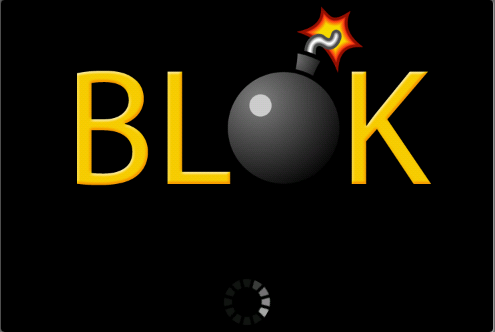
\includegraphics[scale=0.3]{img/1.png} \\
			\end{minipage}\\
		\end{tabular}
		\end{center}

		
	
	\end{frame}
	
	\begin{frame}
	\frametitle{Application}
	\framesubtitle{Chargement de l'application}
		\begin{block}{Premier lancement}
			\begin{itemize}
			 	\item copie des cartes officielles dans le repertoire téléphone 
				\item création de la base de données SQLite
				\item ajouts des cartes dans la base de données
				\item initialisation des tables	systèmes
				\item création compte local et ajout à la base de données
			\end{itemize}
		\end{block}
				
		\begin{block}{Lancement normal}
			\begin{itemize}
				\item chargement de la base de données 
				\item instantiation dernier utilisateur
			\end{itemize}
		\end{block}
	
	\end{frame}
	
	
	\begin{frame}
	\frametitle{Application}
	\framesubtitle{Ecran d'accueil}
		\begin{center}
		\begin{tabular}{cc}
			\begin{minipage}{4cm}
		
				Menu d'accueil
				\begin{itemize}
					\item Partie locale
					\item Partie multijoueur
					\item Editeur de carte
					\item Options
					\item Choix compte local
					\item Ajout compte local
					\item Aide
				\end{itemize}
			\end{minipage}  &		
			\begin{minipage}{8cm}
				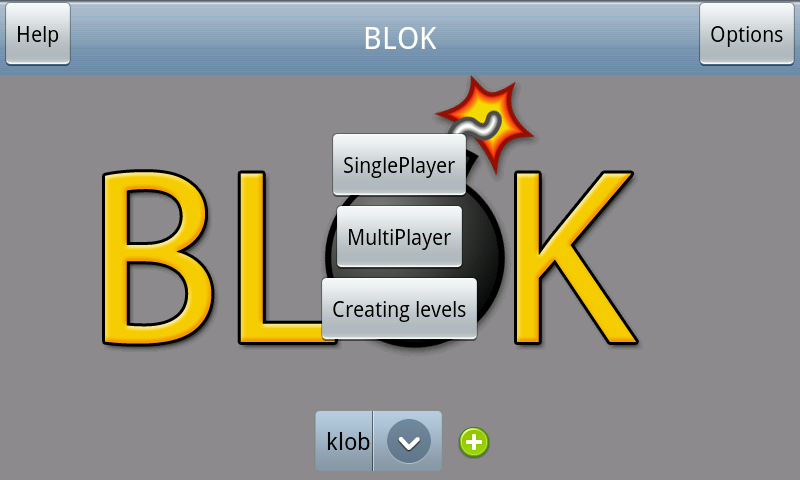
\includegraphics[width=6.5cm]{img/2.png} 
			\end{minipage}\\
		\end{tabular}
		\end{center}
	
	\end{frame}
	
	\begin{frame}
	\frametitle{Application}
	\framesubtitle{Les menus}
	
		\begin{block}{Leurs objectifs:}
			\begin{itemize}
			  \item interface claire et simple
			  \item cohérent
			  \item facile d'utilisation
			  \item navigation intuitive
			  \item ergonomique
			\end{itemize}
		\end{block}
	\end{frame}
	
\subsection{Editeur de cartes}

	\begin{frame}
	\frametitle{Application}
	\framesubtitle{Gestion des ressources}
	
	
	\end{frame}

	\begin{frame}
	\frametitle{Application}
	\framesubtitle{Création ou chargement d'une carte}
	
	\end{frame}
	
	\begin{frame}
	\frametitle{Application}
	\framesubtitle{Moteur de rendu cartes}
	
	\end{frame}
	
	
	\begin{frame}
	\frametitle{Application}
	\framesubtitle{Editeur de cartes}
	
	\end{frame}
	
	\begin{frame}
	\frametitle{Application}
	\framesubtitle{Outils}
	
	\end{frame}
	
	\begin{frame}
	\frametitle{Application}
	\framesubtitle{Exemple de carte}
	
	\end{frame}
	
	\begin{frame}
	\frametitle{Application}
	\framesubtitle{Possibilités finales}
	
	\end{frame}

\subsection{Jeu}
	
	\begin{frame}
	\frametitle{Application}
	\framesubtitle{Création d'une partie solitaire}
	
		\begin{tabular}{cc}
			\begin{minipage}{5cm}
				Création d'une partie solitaire
				\begin{enumerate}
					\item Choix de la carte
					\item Type de la partie
					\item Difficulté des ennemis
					\item Nombre d'ennemis
					\item Temps de la partie
					\item Retourner à l'écran d'accueil
					\item Créer la partie
				\end{enumerate}
			\end{minipage} &
			\begin{minipage}{7cm}
				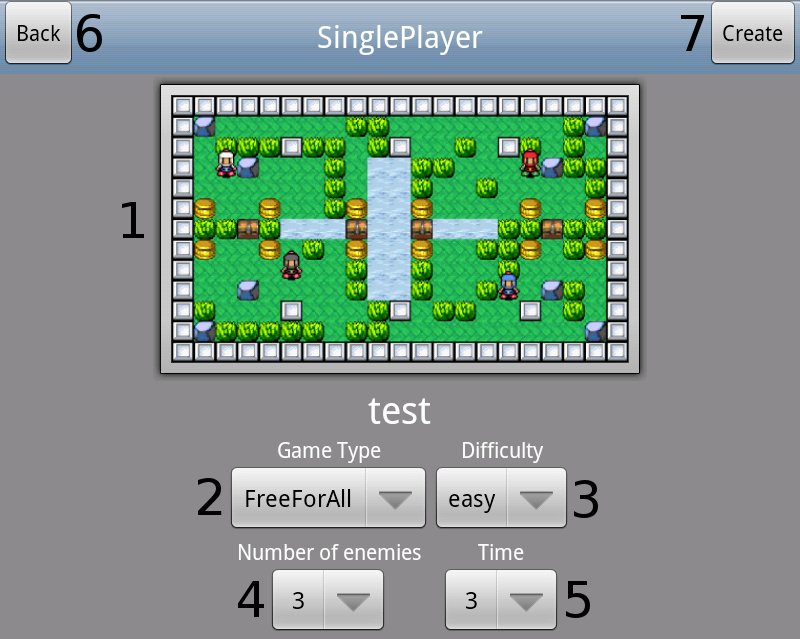
\includegraphics[width=6cm]{img/singleplayerbis.png} 
			\end{minipage}\\
		\end{tabular}
	
	\end{frame}
	

	\begin{frame}
	\frametitle{Application}
	\framesubtitle{Intelligence artificielle}
	
		\begin{tabular}{cc}
			\begin{minipage}{4cm}
				Niveaux de difficulté
				\begin{enumerate}
					\item Facile
					\item Moyen
					\item Difficile
				\end{enumerate}
			\end{minipage} &
			\begin{minipage}{6cm}
				
\includegraphics[width=6cm]{img/bots.png} 
			\end{minipage}\\
		\end{tabular}
	
	\end{frame}
	
	\begin{frame}
	\frametitle{Application}
	\framesubtitle{Pathfinding}
	
		\begin{tabular}{cc}
			\begin{minipage}{5cm}
				Algorithme A*
				\begin{enumerate}
					\item Heuristique (de Manatan)
					\item Coût de deplacement
					\item Premier chemin trouvé
					\item Rapidité (Dijskra)
				\end{enumerate}
			\end{minipage} &
			\begin{minipage}{5cm}
				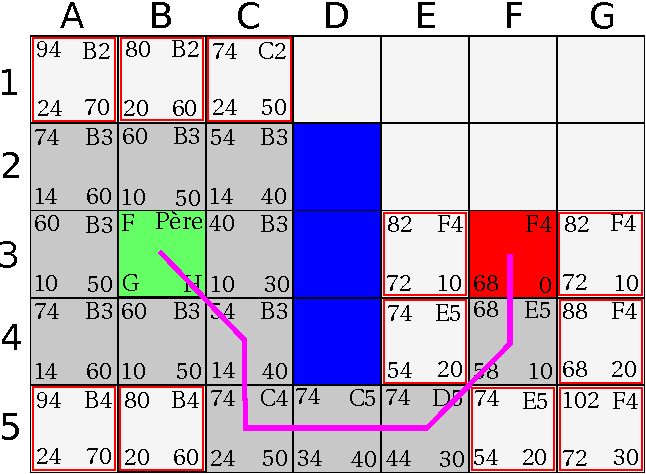
\includegraphics[width=6cm]{img/astar.png} 
			\end{minipage}\\
		\end{tabular}
	
	\end{frame}
	
	\begin{frame}
	\frametitle{Application}
	\framesubtitle{Pathfinding}
	
		\begin{tabular}{cc}
			\begin{minipage}{5cm}
				Algorithme de parcours en largeur
				\begin{enumerate}
					\item Pas de case d'arrivé necessaire
					\item Tous les chemins possibles
					\item Premier chemin trouvé
					\item Rapidité
				\end{enumerate}
			\end{minipage} &
			\begin{minipage}{5cm}
							\begin{center}
				\begin{tabular}{|c|c|c|c|c|c|c|} \hline
				\rowcolor{gray}  &  &                    &  &                  &  &                   \\\hline
				\cellcolor{gray} & \cellcolor{orange}1 $\leftarrow$ & \cellcolor{green}1 $\leftarrow$                   &&                && \cellcolor{gray} \\\hline
				\cellcolor{gray} & \cellcolor{orange}1 $\leftarrow$ & \cellcolor{gray}   & \cellcolor{gray} & \cellcolor{gray} &&	\cellcolor{gray} \\\hline
				\cellcolor{gray} & \cellcolor{orange}1 $\leftarrow$ & \cellcolor{orange}1 & \cellcolor{orange}1 $\rightarrow$ & \cellcolor{red}O                 && \cellcolor{gray} \\\hline
				\cellcolor{gray} & \cellcolor{orange}1 $\leftarrow$ & \cellcolor{gray}   & \cellcolor{gray} & \cellcolor{gray} && \cellcolor{gray} \\\hline
				\cellcolor{gray} & \cellcolor{red}O &                  &  &                && \cellcolor{gray} \\\hline
				\cellcolor{gray} && \cellcolor{gray}   && \cellcolor{gray} &&	\cellcolor{gray} \\\hline
				\cellcolor{gray} &&                  &&                && \cellcolor{gray} \\\hline
				\rowcolor{gray}  &  &                    &  &                  &  & \\\hline
				\end{tabular}
			\end{center}
			\end{minipage}\\
		\end{tabular}	
	
	\end{frame}
	
	\begin{frame}
	\frametitle{Application}
	\framesubtitle{Moteur de rendu}
	
		\begin{tabular}{ccccc}
			\begin{minipage}{3cm}
				\begin{center}
					Image
				\end{center}		
			\end{minipage} & &
			\begin{minipage}{2cm}
				\begin{center}
					Hashmap
				\end{center}
			\end{minipage} & &
			\begin{minipage}{3cm}
				\begin{center}
					Resultat
				\end{center}
			\end{minipage}\\
			\begin{minipage}{3cm}
				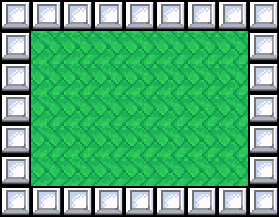
\includegraphics[width=3cm]{img/bitmap.png}
			\end{minipage} & + &
			\begin{minipage}{2cm}
				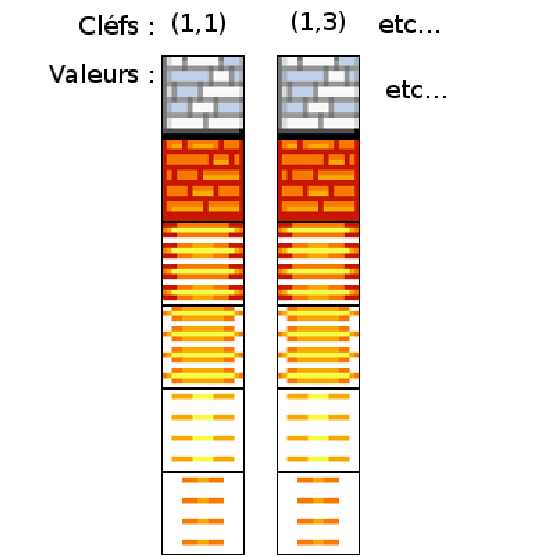
\includegraphics[width=3cm]{img/hashmap.png} 
			\end{minipage} & = &
			\begin{minipage}{3cm}
				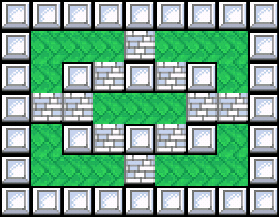
\includegraphics[width=3cm]{img/map.png} 
			\end{minipage}\\
		\end{tabular}
	
	\end{frame}
	
	\begin{frame}
	\frametitle{Application}
	\framesubtitle{Moteur Physique}
	
	\end{frame}
	
		\begin{frame}
	\frametitle{Application}
	\framesubtitle{Le jeu}
	
		\begin{tabular}{cc}
			\begin{minipage}{3cm}
				Ecran de jeu
				\begin{enumerate}
					\item 
				\end{enumerate}
			\end{minipage} &
			\begin{minipage}{7cm}
				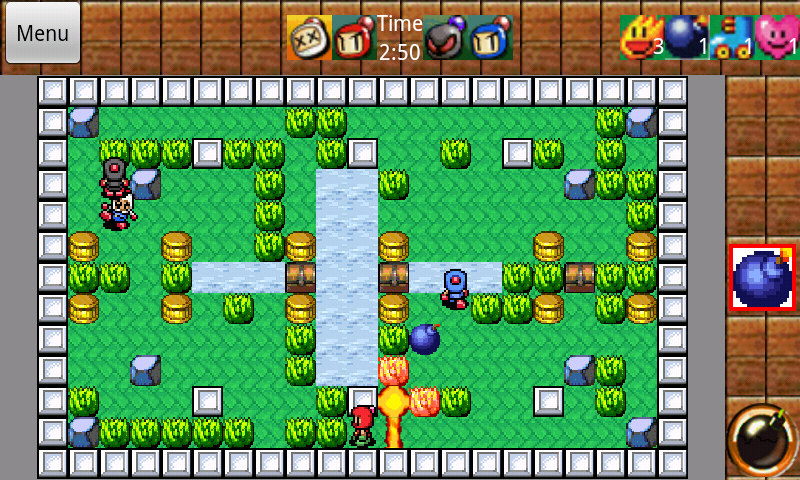
\includegraphics[width=8cm]{img/game.png} 
			\end{minipage}\\
		\end{tabular}
	
	\end{frame}
	
	\begin{frame}
	\frametitle{Application}
	\framesubtitle{Multitouch}
	
	\end{frame}
	
	\begin{frame}
	\frametitle{Application}
	\framesubtitle{Menu}
	
			\begin{tabular}{cc}
			\begin{minipage}{3cm}
				Menu
				\begin{enumerate}
					\item Reprendre
					\item Options
					\item Redemarrer
					\item Quitter
				\end{enumerate}
			\end{minipage} &
			\begin{minipage}{8cm}
				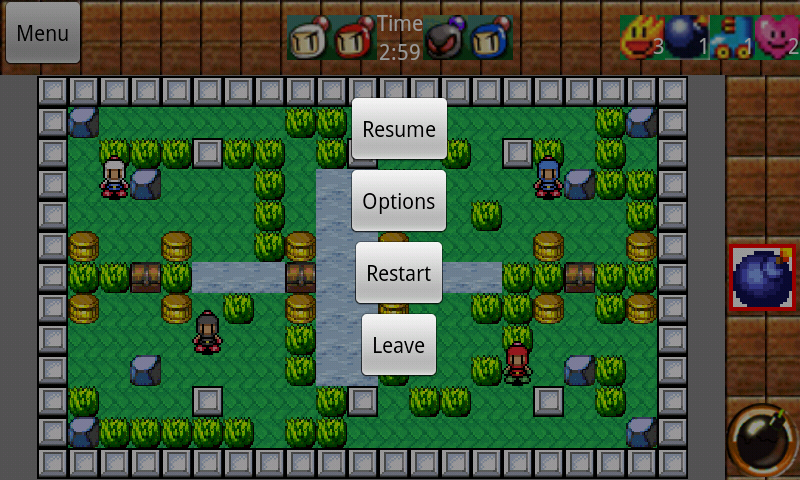
\includegraphics[width=8cm]{img/menusolo.png} 
			\end{minipage}\\
		\end{tabular}
	
	\end{frame}

\subsection{Reseau}

\begin{frame}
\frametitle{Application}
\framesubtitle{Fonctionnalités}

	\begin{center}
		\begin{tabular}{cc}
			\begin{minipage}{4cm}
				Les joueurs ont accès à:
				\begin{itemize}
				  \item création compte multijoueur
				  \item connexion compte
				  \item listage de parties en lignes
				\end{itemize}
				\end{minipage}&		
				
			\begin{minipage}{8cm}
				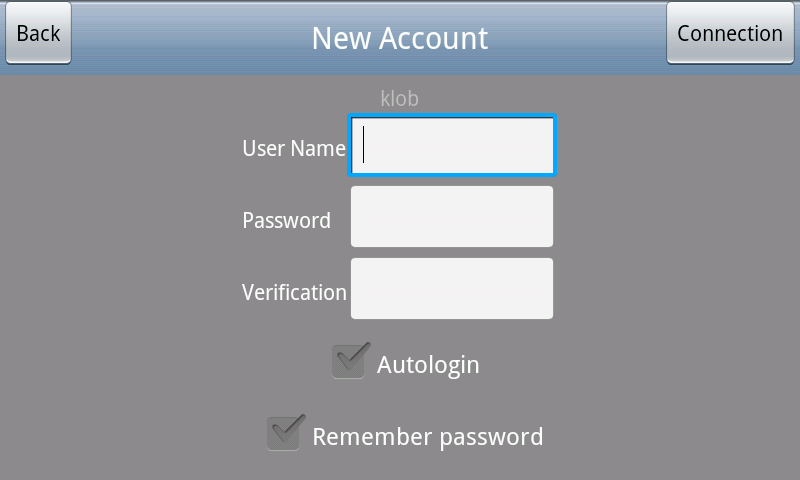
\includegraphics[width=7cm]{img/3.png} 
			\end{minipage}\\
			
			
			\end{tabular}
	\end{center}
	

\end{frame}

\begin{frame}
\frametitle{Application}
\framesubtitle{Outils}
	\begin{center}
		\begin{tabular}{cc}
			\begin{minipage}{7cm}
			
			\begin{block}{Outils utilisés: }
				\begin{itemize}
				  \item servlet
				  \item serveur d'application
				  \item JSON
				  \item SQLite
				\end{itemize}
			\end{block}
			
			\end{minipage}&
			
			\begin{minipage}{4cm}
				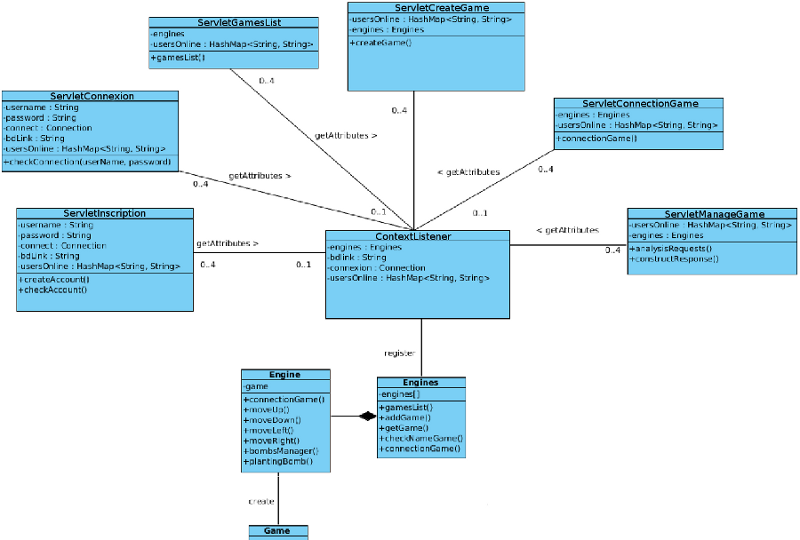
\includegraphics[scale=0.5]{img/serveur.png} 
			\end{minipage}\\
				
			\end{tabular}
	\end{center}
			
\end{frame}


\begin{frame}
\frametitle{Application}
\framesubtitle{Principes}

	\begin{center}
		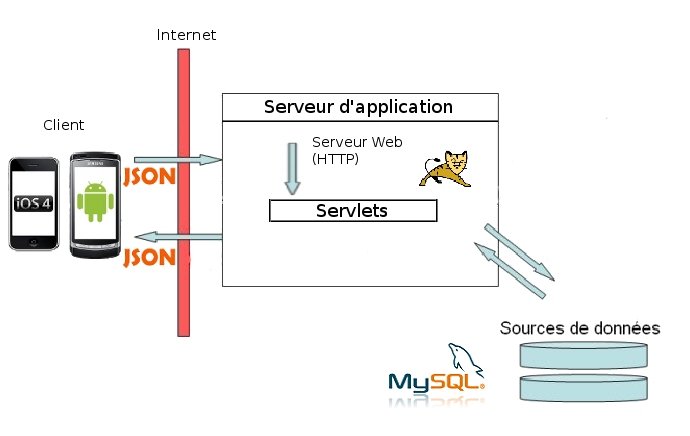
\includegraphics[width=9.4cm]{img/4.png} 
	\end{center}
	

\end{frame}
